\documentclass{beamer}

\mode<presentation>
{
  \usetheme{Madrid}     
  \usecolortheme{default}
  \usefonttheme{professionalfonts}
  \setbeamertemplate{navigation symbols}{}
  \setbeamertemplate{caption}[numbered]
} 

\newcommand{\source}[1]{\begin{textblock*}{4cm}(8.7cm,8.6cm)
    \begin{beamercolorbox}[ht=0.5cm,right]{framesource}
        \usebeamerfont{framesource}\usebeamercolor[fg]{framesource} Source: {#1}
    \end{beamercolorbox}
\end{textblock*}}
\setbeamercolor{framesource}{fg=gray}
\setbeamerfont{framesource}{size=\tiny}
\usepackage[absolute,overlay]{textpos}
\usepackage[english]{babel}
\usepackage[utf8]{inputenc}
\usepackage{xcolor}
\usepackage{pgfpages}
\usepackage{setspace}
\pgfpagesuselayout{resize to}[%
  physical paper width=8in, physical paper height=6in]


\title[Mathematics Department]{Persistent Homology}
\author{Sunay Doğan}
\institute{METU}
\date{}

\begin{document}

%------------------------------
\section{Title}
\begin{frame}
    \titlepage
\end{frame}
%------------------------------
\section{Outline}
\begin{frame}{Outline}

    \begin{enumerate}
        \item Introduction
        \item Fundamental Concepts
        \item Introduction to Persistent Homology
        \item Examples
        \item References
    \end{enumerate}
    
\end{frame}

%----------------------------------
\section{Introduction}
\begin{frame}{Introduction}
    Persistent homology, as a tool in topological data analysis (TDA), studies topological features of a sample data set at different scales to understand the topological characteristic of the underlying space.\\
    \vspace*{0.5cm}
    The key idea is this: Topological aspects of the sample data set that \underline{persist} as the scale grows can give us an understanding about the topology of population data set. 
\end{frame}
%------------------------------------------

\section{Fundamental Concepts}
\begin{frame}{Fundamental Concepts - Simplicial Complexes}
    Given $n+1$ affinely independent points in $\mathbb{R}^{n+1}$, $\Delta^{n} = \{(t_0,t_1,...,t_n)\in \mathbb{R}^{n+1} : \sum\limits_{i=0}^{n}t_i=1, t_i \geq 0\}$
    is called a \textcolor{red}{standard n-simplex}. Simplices are generalizations of triangles in any dimension.

    \vspace{0.5cm}
    Let $V$ be a vertex set such that 
    \begin{enumerate}
        \item $\forall S\subseteq V$, for any element $\sigma \in S$, all subsets of $\sigma$ are in $S$ and
        \item If for any $\sigma,\tau \in S$, then $\sigma \cap \tau \in S$.
    \end{enumerate}
    Then V is called an \textcolor{red}{abstract simplicial complex}. Simplicial complexes are triangluable spaces. 

\end{frame}

%-----------------------------------------

\begin{frame}{Fundamental Concepts - Chain Complexes}
    Let $V_k$ denote the set of all $k$-simplices of V. Then, $\sum\limits_{i=1}^Nr_i\sigma_i$ for $\sigma \in V_k$ and $r_i \in \mathbb{Z}$ is called a \textcolor{red}{simplicial k-chain}. \\

    \vspace{0.5cm}
    The map $\partial_n: V_n \rightarrow V_{n-1}$ such that 
    $\partial_n(\sigma) = \sum\limits_{i}(-1)^i(v_1,...,\hat{v_i},...,v_n)$
    where $\sigma = (v_1,...,v_n)$ is called \textcolor{red}{boundary operator}. Boundary operators satisfy $\partial_{k-1}\circ \partial_{k}=0$  $\forall k$.\\

    \vspace{0.5cm}
    The sequence $...V_{k+1} \xrightarrow{\partial_{k+1}} V_k \xrightarrow{\partial_{k}} V_{k-1}...$ is a \textcolor{red}{chain complex}.
    
\end{frame}

\begin{frame}{Fundamental Concepts - Homology}
    \textcolor{blue}{Notice:} $Im(\partial_{k+1})\subseteq Ker(\partial_{k})$. \\
    \vspace{0.5cm}
    \textcolor{red}{$k^{th}$ homology} of $V$ is defined as $H_k = Z_k/B_{k+1}$ where $Z_k:=Ker(\partial_k)$ and $B_{k+1}:=Im(\partial_{k+1})$. \\
    \vspace{0.5cm}
    If $\alpha$ is a $k$-chain such that $\partial_k(\alpha) = \emptyset$ then $\alpha \in Z_k$ is called a \textcolor{red}{$k$-cycle}. If there exists a $(k+1)$-chain $\beta$ such that $\partial_{k+1}(\beta)=\alpha$ then $\alpha \in B_{k+1}$ is called a \textcolor{red}{$k$-boundary}. \\
    \vspace{0.5cm}
    Intuitively, $k^{th}$ homology measures $k$-cycles of space which are not boundary of a region. The \textcolor{red}{$k^{th}$ Betti number} $\beta_k=rank(H_k)$ is the number of $k$ dimensional holes of simplicial complex V.
\end{frame}

\section{Persistent Homology}
\begin{frame}{Persistent Homology}
    Let $X$ be a finite set of sample data. Our purpose is to construct simplicial complexes, $K^{\delta}$ using elements of $X$, for any given $\delta \in \mathbb{R}$ such that if $m \leq n$ then $K^m \subseteq K^n$. This ordered set of simplicial complexes is called \textcolor{red}{filtration}.\\
    \vspace{0.5cm}
    As simplicial complexes transform from one another, some holes may appear (birth) and some others disappear (death). Persistence homology examines lifespan (\textcolor{red}{persistance barcode}) of holes. 
\end{frame}

\begin{frame}{Persistent Homology}
    \begin{figure}
        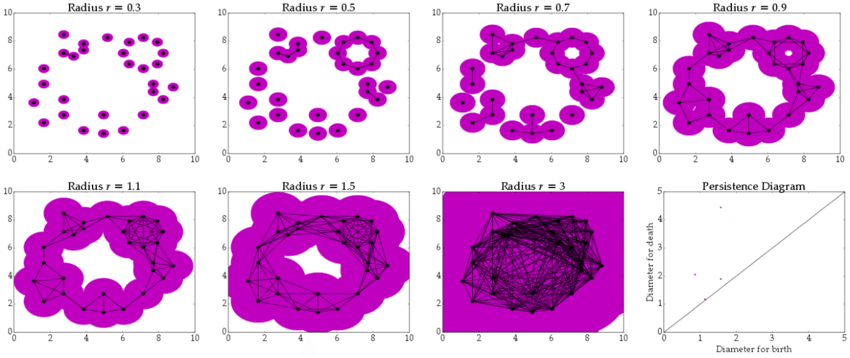
\includegraphics[scale=0.4]{./example.png}
        \source{Munch, Elizabeth. (2017). A User’s Guide to Topological Data Analysis. Journal of Learning Analytics. 4. 47-61. 10.18608/jla.2017.42.6. }
        \caption{An example of filtration}
    \end{figure}
\end{frame}


\begin{frame}{Persistent Homology}
    $H^{\delta,p}_k = Z^{\delta}_k/(B^{\delta+p}_k \cap Z^{\delta}_k)$ is called \textcolor{red}{p-persistent $k^{th}$ homology} of $K^{\delta}$. \\
    \vspace*{0.5cm}
    Then, the corresponding Betti number is $\beta^{\delta,p}_k=rank(H^{\delta,p}_k)$. This is the number of holes that persist (neither birth nor death) during the interval $(\delta,\delta+p)$.
\end{frame}

\begin{frame}{Persistence Diagrams}
    For a simplicial complex, let $[s,t)$ represents its persistence barcode. Here $\delta=s$ is the birth and $\delta=t$ is the death. Then, each point $(s,t)$  has a \textcolor{red}{multiplicity $n_{s,t}$} which is the number of simplicial comlexes that "lived" in the interval $[s,t)$. \\
    \vspace{0.5cm}
    \textcolor{red}{Persistence diagram} is the set of points (s,t), with multiplicities $n_{s,t}$ such that $0 \leq s < t \leq n+1$ where $n$ is the largest value of $\delta$.
\end{frame}

\begin{frame}{Persistence Diagrams (Example)}
    \begin{figure}
        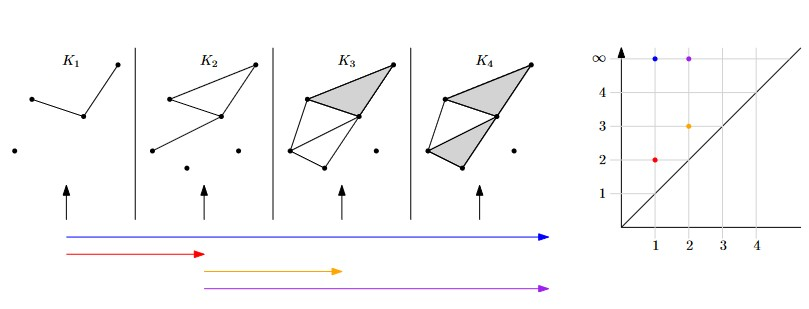
\includegraphics[scale=0.55]{./diagram.jpg}
        \source{Ž. Virk. Introduction to Persistent Homology. Založba UL FRI, University of Ljubljana, 2022, doi: 10.51939/0002. }
        \caption{Persistence barcodes and persistence diagram}
    \end{figure}
\end{frame}

\begin{frame}{Fundamental Lemma of Persistent Homology}
    $\beta_{s,t}=\sum\limits_{}$
\end{frame}   
\end{document}